\chapter{Top-Down Approach}
\section{Change Point Detection}
For this approach, the data was split into non-overlapping segments for
featurization using techniques from the statistical field of change point detection.
These techniques have found wide application in control theory and other disciplines
that require analysis of time series data of dynamic systems (REF).
Change point detection assumes that (COME BACK TO THIS). To figure out when these
changes occur, a \emph{score} is generated for each time tick, and if the score is
above a given threshold a change is predicted to have occurred between that tick
and its immediate predecessor. To generate a score at
a time tick, we compare a window of data that immediately preceeds it (the
\emph{reference data}) and it along with a window of data that immediately follows it
(the \emph{test data}). (SHOULD COMPARE FIXED LENGTH TO VARIABLE LENGTH
REFERENCE AND TEST WINDOWS, AND NOTE THAT IT MAY BE IMPOSSIBLE TO PREDICT CHANGES
FOR THE FIRST FEW AND LAST FEW TICKS) (PICTURE).

Model-based approaches to change point detection assume that each tick in
a time series is a draw from some underlying probability distribution.
Scores are generated by estimating the distribution of the reference data
and the test data, and then by calculating in some fashion the likelihood
that the test data belongs to the that distribution.
If it is reasonable to assume that the data belongs to a particular
family of distributions then parametric estimation methods can be used,
otherwise estimation will be non-parametric. Distance-based
approaches generate scores through other metrics of dissimilarity or
distance between the reference data and the test data. Notationally,
we say that for each tick $i$ in a time series:

\[
s_i = D(x_{ref,i}, x_{test,i})
\]

Where $s_i$ is the score of the $i$th tick, $x_{ref,i}$ is the reference
data associated with the $i$th tick, $x_{test,i}$ is the test data
associated with the $i$th tick, and $D(A,B)$ is a function that computes the
dissimiliarity between a matrix of data $A$ and matrix of data $B$, and is
particular to the given change point algorithm.

There are many different modeling assumptions and associated algorithms
for generating change point detection scores. The Control Chart
method assumes that the reference data is drawn from a
multivariate normal distribution, and scores are calculated from the Mahalanobis
distance of the given tick from the estimated multivariate normal:

\[
s_i = \sqrt{(\bar{x}_{ref,i} - x_i)^T \, S_{ref,i}^{-1} \, (\bar{x}_{ref,i} - x_i)}
\]

where $\bar{x}_{ref,i}$ is the sample mean of the reference data, $S_{ref,i}$
is the sample covariance matrix of the reference data, and $x_i=x_{test,i}$ is
the $i$th data point.



Kernel Density Estimation,
Exponential Weighted Moving Average, CUSUM
(TODO: include more and explain them more).

\section{Methodology}
We were particularly interested in testing the performance of the
Kullback-Leibler Importance Estimation Proceedure (KLIEP).
This non-parametric approach generates scores using the Kullback-Leibler
divergence between the reference data and the test data. However, instead of
estimating the density of the reference distribution and test distribution
separately, and then comparing them with a likelihood ratio, it models and
estimates the likelihood ratio directly with a Gaussian kernel. Cross-validation 
set the kernel width $\sigma$ at each individual time tick.
We tested this algorithm using a module that was previously implemented in Matlab.
Our reference windows were fixed at a length of 10 seconds, and our test
windows were fixed at a length of 1 second.

We also tested the simpler Control Chart algorithm as a baseline. This
algorithm assumes that each time tick is a draw from a multivariate normal distribution.
It is assumed that no changes occur in the reference window, and the score of a time
tick is the Mahalonobis distance of the tick from the estimated distribution of its reference data.
The mean vector and covariance matrix of the reference data is estimated using
the sample mean and sample standard deviation along each of the 3 axes. For simplicity
we assumed that the covariance between pairs of axes is 0, so the covariance matrix is
diagonal. Our reference windows were fixed at a length of 10 seconds. 

Threshold values were chosen by considering a number of false positive rates of
the change point detection algorithms. A smaller false positive rate per second
corresponded to a higher and more conservative threshold, which split the
time series into fewer segments for featurization. A larger false positive rate
corresponded to a lower threshold, which split the time series into more segments.
The false positive rates that we tested ranged from 0.005 per second to 0.5 per second (EXPAND).

\section{Results}
To measure the performance of a time series classification algorithm we used
two metrics. Accuracy is defined as the number of
ticks that an algorithm correctly classifies in a time series, over the total number of ticks
in the time series. In many applications involving streaming accelerometer data
it is important to quickly detect changes in activity type in real time, so we
were also interested in our algorithms'' detection time.
Detection time is defined as the average number of ticks
required for the algorithm to begin correctly classifying data after a
true activity change has occurred.

As shown in Figure 2.1, we plotted accuracy and detection time as a function of the allowed
false positive rate per second, along with plots of accuracy against detection
time, for the SVM, Decision Tree, and Neural Net classifiers.

\begin{figure}
 \centering
 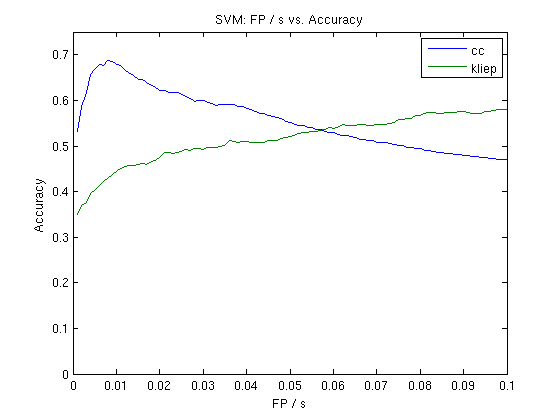
\includegraphics[scale=0.3]{svm_fps_acc.png}
 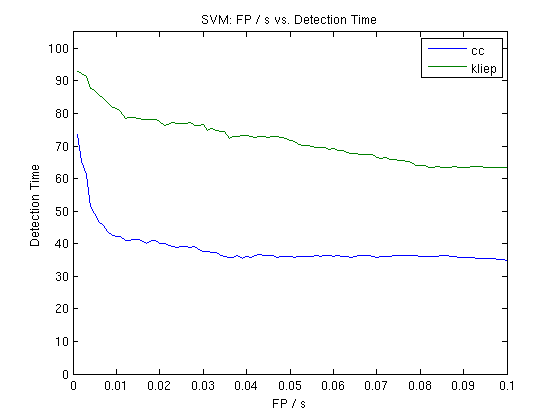
\includegraphics[scale=0.3]{svm_fps_det.png}
 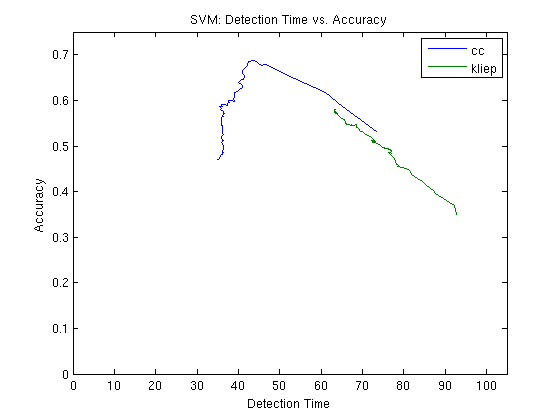
\includegraphics[scale=0.3]{svm_det_acc.png}
 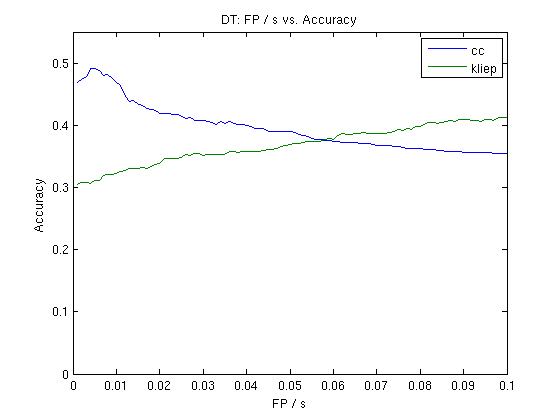
\includegraphics[scale=0.3]{dt_fps_acc.png}
 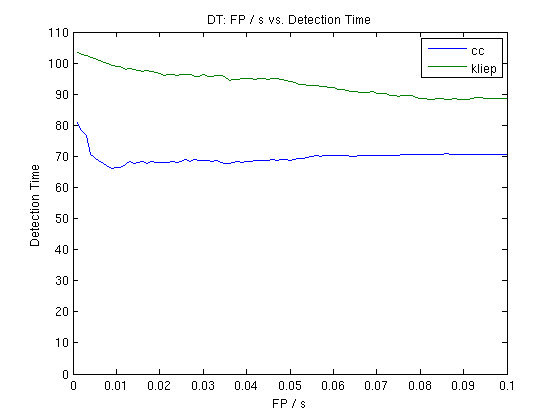
\includegraphics[scale=0.3]{dt_fps_det.png}
 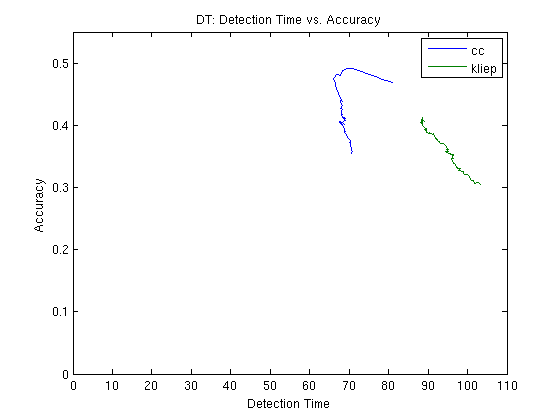
\includegraphics[scale=0.3]{dt_det_acc.png}
 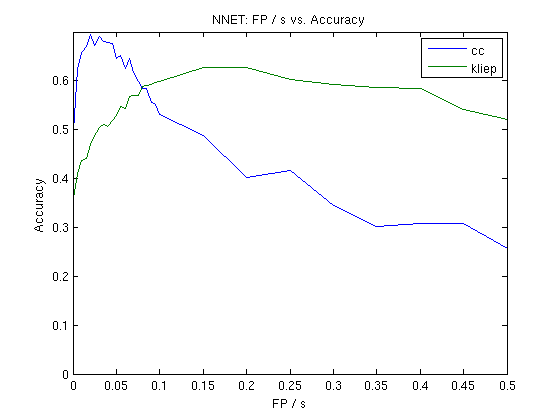
\includegraphics[scale=0.3]{nnet_fpr_acc.png}
 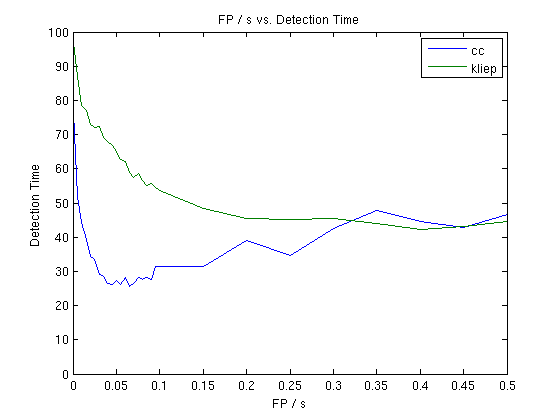
\includegraphics[scale=0.3]{nnet_fpr_det.png}
 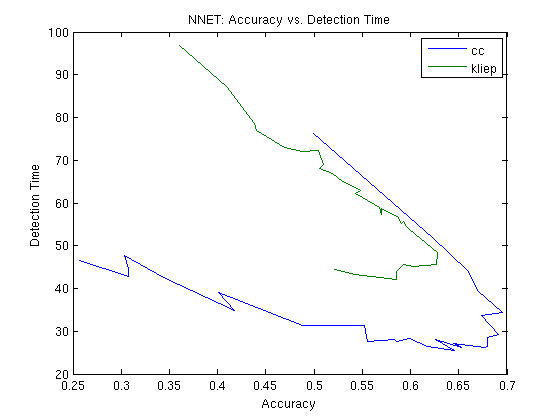
\includegraphics[scale=0.3]{nnet_acc_det.png}
 \caption{CPD Classification Performance}
\end{figure}
